%----------------------------------------------------------------------------------------
%	PART III
%----------------------------------------------------------------------------------------

\part{Nyxi Sciences}

%----------------------------------------------------------------------------------------
%	Tenebrivity
%----------------------------------------------------------------------------------------

\chapterimage{placeholder.png} % Chapter heading image

\chapter{Tenebrivity}

One of the most significant impacts that the Nyxi had on human civilization was
a full understanding of what we used to call dark matter. At the time, in spite
of hundreds of years of research, humanity was still unable to make any
progress understanding dark matter beyond theoretical pursuits, especially
since we lacked any significantly accessible dark matter to attempt more
advanced measurements or any experiments. Meanwhile, we learned that the
Nyxophora is abundant with dark matter, to the extent that it's even used in
the biochemistry of the Nyxi. After first contact and overcoming the
difficulties of communication, one of the first provisions from the Nyxi was a
full explanation of dark matter, which is now referred to as tenebrum, and an
abundance of access to it. While it took quite some time to understand their
theory in the context of humanity's framework of physics, the final result -
the Theory of Tenebrivity - revolutionized our understanding of the universe
and our technological capabilities.

The complete theory is organized hierarchically by scale, extending all of our
prior models of the universe. From the smallest to largest scales, the theory's
components are described by:
\begin{description}
  \item[Fractolet-T Theory] The extension of Fractolet Theory, the current most
    fundamental Theory of Everything, extended to include additional
    semidimensional stabilian and diffusian fractolets that interact to create
    umbristrings and tenebranes.
  \item[Tenebrivic Fractobrane-String Theory] The theory that describes how
    umbristrings and tenebranes resonate and interact to form the quantum
    tenebrivic particle fields.
  \item[Quantum Tenebridyanmics] The quantum field theory of tenebrivic particles. This
    theory explains the fundamental tenebrivic force, the composite particles
    formed from confinement, and the fundamental model of atomoxes - atom-like
    structures formed by tenebrivic particles.
  \item[Tenebrichemistry] The full theory of how differing atomoxes form the
    netherelements, which in turn form the nethermolecules, and the resulting
    chemical interactions.
  \item[Tenebrum Dynamics] The human-scale study of tenebrum and its properties,
    especially in relation to the mechanics of lux matter.
  \item[Tenebrivic Cosmology] The impact that tenebrum has had on the structure and
    evolution of the universe.
\end{description}

A deep treatise of the two smallest-scale theories are well beyond the scope of
this book and require an extensive background in theoretical physics, but we'll
briefly review the concepts included. Beyond that, we'll then go into the
essential formalism of each theory which will serve as an effective
introduction if you wish to dive deeper into the relevant branch of science.

\section{Fractolets, Umbristrings, Tenebranes}

\chapterimage{placeholder.png} % Chapter heading image

\chapter{Quantum Tenebridynamics}
In modern theoretical physics, \textbf{quantum tenebridynamics} (\textbf{QTD}) is the theory of the the tenebrivic interactions between \textbf{noxions} and \textbf{thuleons} mediated by \textbf{xenobrons} and \textbf{vanibrons}. Noxions are fundamental particles that make up composite diombrons such as the protombron and neutrombron. Thuleons are also fundamental particles that make up exotic matter which enables several superluminal technologies. The QTD analog of electric charge is a property called \textit{tenebridge}. Unlike electric charge with can have two types of values (positive, negative), tenebridge can have \textit{four} types of values. These types receive labels from the classical elements in Nyxi antiquity:
\begin{center}vortex, crystal, flow, and spark.\end{center}

Xenobrons are vanibrons are the force carriers of the theory, with xenobrons having analogous properties to the photon in quantum electrodynamics, and vanibrons having analogous properties to the gluon in quantum chromodynamics.
\begin{table}[ht]\label{QTDParticles}
  \centering
  \begin{tabular}{c c c c c c}
    \toprule
    \textbf{Particle} & \textbf{Field}                             & \textbf{Tenebridgials} & \textbf{Type} & \textbf{Spin} & \textbf{Mass} \\
    \midrule
    \textbf{Xenobron} & $\xenfield{\mu}$                           & 0                      & boson         & 1             & 0             \\[10pt]
    \textbf{Noxion}   & $\noxfield{\sigma}{\alpha}$                & 1                      & fermion       & 1/2           & 0             \\[10pt]
    \textbf{Vanibron} & $\vanfield{\mu}{\alpha}{\beta}$            & 2                      & boson         & 1             & 0             \\[10pt]
    \textbf{Thuleon}  & $\thufield{\sigma}{\alpha}{\beta}{\gamma}$ & 3                      & fermion       & 3/2           & $\pm m_{t}$   \\
    \bottomrule
  \end{tabular}
  \caption{Summary of Particles in QTD}
\end{table}
In mathemtically formal language, QTD is a type of quantum field theory called a non-abelian gauge theory, with symmetry group U(1) \texttimes SU(4). The theory is an important part of the Universal Model of particle physics. Research on QTD was blocked for the majority of human history, and became accessible after humanity's first contact with the Nyxi.

\section{History}
From the early 21st century to the 41st century, the prevailing consensus within the scientific community posited the existence of a theoretical form of matter that constituted approximately 85\% of the universe's total matter content. This enigmatic substance came to be known as "dark matter." Its name stems not only from its elusive nature, rendering it imperceptible to direct observation, but also due to its negligible interactions with conventional baryonic matter. Further complicating the matter was the absence of a copious, proximate concentration of dark matter, inhibiting more intimate studies. This scarcity stands in stark juxtaposition to the conditions on Nyx, where the abundance of dark matter in Nyxophora was so profound that it played integral roles in both biological and planetary processes of the Nyxi civilization.

As human civilizations evolved, so did their understanding of the cosmos. One of the most transformative events in the annals of scientific progress occurred during the early 4000s, marked by a pivotal collaboration with the Nyxi species. This interspecies partnership, based on shared intellectual curiosity and the promise of mutual enlightenment, propelled humanity's comprehension of what was once termed `dark matter' to new, unparalleled heights.

Following this collaboration, "dark matter" was subsequently rebranded as "tenebrivic matter." The renaming was emblematic, not just of a newfound understanding, but also of a paradigm shift in the way scholars approached this mysterious substance. With the Nyxi's unique, experiential knowledge, which was rooted in their own planet's profusion of this matter, and the combined cerebral prowess of both species, the field of quantum tenebridynamics emerged. This discipline elucidated the fundamental principles governing the interactions of tenebrivic matter at the quantum level, a subject hitherto unexplored due to the previously mentioned scarcity of the substance in our own vicinity.

The ripened comprehension of tenebrivic matter bore fruits beyond mere academic pursuits. Technological innovations, unimaginable even in the wildest dreams of prior generations, emerged from this golden age of understanding. The theories postulated and validated under quantum tenebridynamics laid the groundwork for the development of warp drive and wormhole technology. These advancements revolutionized space travel, reducing interstellar journeys from lifetimes to mere hours. Humanity was no longer tethered to the confines of our solar system; the vastness of the universe lay invitingly open for exploration.

But perhaps, even more significant than the technological renaissance, was the answer to a question that had long confounded astronomers and cosmologists: Why was the universe's expansion accelerating at such an exponential rate? It was discovered that a subtype of tenebrivic matter, dubbed thuleonic matter, possessed a unique property of negative mass. This peculiarity led to a phenomenon described as the "runaway effect". In essence, the presence of thuleonic matter, with its counterintuitive gravitational influence, drove galaxies apart at increasing velocities. This revelation not only offered a solution to the cosmic expansion conundrum but also opened up an entirely new frontier of inquiry into the nature of mass, gravity, and the ultimate fate of the universe.

In retrospection, the collaboration with the Nyxi wasn't merely an exchange of knowledge. It represented an intermingling of cosmic perspectives and a mutualistic journey towards unraveling the enigmas of existence. Through shared endeavor, the universe became less opaque, its mysteries slightly less mystifying, ushering in the Tenebrivic Epoch — a period of enlightenment, progress, and infinite possibilities.

\section{Symmetries}
Every field theory of particle physics is based on certain symmetries of nature whose existence is deduced from observations. The group symmetry U(1) \texttimes SU(4) corresponds to the local symmetry whose gauging gives rise to QTD\@. Symmetries are so crucial to field theories because each symmetry is associated with a the conservation of some physical observable. Throughout QTD, we will see that the conserved property is tenebridge.

\subsection{U(1) Symmetry}
U(1) symmetry refers to a type of continuous symmetry associated with the group of complex numbers of magnitude 1 (or, equivalently, the group of 2x2 unitary matrices with determinant 1). This might sound abstract at first, but let's unpack it with a bit of mathematics and then provide some tangible examples.

A complex number is written as \(z = a + bi\), where \(i\) is the imaginary unit. The magnitude (or modulus) of this number is given by:
\[\left| z \right| = \sqrt{a^2 + b^2}\]

The group ``Unitary 1'' - U(1) - consists of all complex numbers for which \(\left|z\right|=1\). That is, they lie on the unit circle in the complex plane. Each of these numbers can be expressed as:
\[z=e^{i\theta}\]
where \(\theta\) is a real number (angle in radians). As you change \(\theta\), you trace out the unit circle. The symmetry refers to the fact that you can change \(\theta\) by any amount and still remain within the U(1) group. This continuous change is why it's called a continuous symmetry.

\begin{example}[U(1) Symmetry in Everyday Life]
  Consider an object spinning around an axis. The object's dynamics remain invariant under rotations about this axis, and these rotations can be described by a U(1) symmetry. The associated conserved quantity here is the component of angular momentum along the axis of rotation.
\end{example}

U(1) symmetry arises from the interactions between the noxions and xenobrons. Mathematically, you can change the phase of the of the quantum wavefunction of a particle with tenebridge by any amount (which corresponds to a U(1) transformation), and the equations of tenebrivity remain unchanged. This symmetry leads to the conservation of tenebridge \textit{magnitude}.

\begin{example}[U(1) Conservation]
  A spark-noxion \(n_s\) and flow-noxion \(n_f\) approach each other and then repel. This is mediated by the tenebridgeless-xenobron:
  \begin{itemize}
    \item The first noxion emits a xenobron:\\
          \(n_s \rightarrow n_s + x\)
    \item The second noxion absorbs a xenobron:\\
          \(n_f + x \rightarrow n_f\)
    \item An external observer just sees the noxions repel:\\
          \(n_s + n_f \rightarrow n_s + n_f\)
  \end{itemize}
  Throughout each step, the magnitude of tenebridge was conserved:
  \begin{itemize}
    \item \(1 = 1 + 0\)
    \item \(1 + 0 = 1\)
    \item \(1 + 1 = 1 + 1\)
  \end{itemize}
\end{example}

\subsection{SU(4)}
The SU(4) symmetry is slightly more intricate than U(1), but the general idea is analogous. ``SU'' stands for ``Special Unitary'', and the number following ``SU'' indicates the dimensionality of the matrices involved. So, SU(4) refers to the group of 4x4 special unitary matrices.

A unitary matrix \(U\) has the property that its adjoint (or conjugate transpose) is its inverse. That is:
\[U^{\dag}U=UU^{\dag}=\mathbb{1}\]
where \(\mathbb{1}\) is the identity matrix. The ``special'' in ``Special Unitary'' refers to the constraint that the matrices have a determinant of 1.

\begin{example}[SU(4) Symmetric Matrix]
  An example of an SU(4) matrix is:
  \[
    M=\frac{1}{2}
    \begin{pmatrix}
      \fourrow{0}{1-i}{0}{0} \\
      \fourrow{1+i}{0}{0}{0} \\
      \fourrow{0}{0}{0}{1-i} \\
      \fourrow{0}{0}{1+i}{0}
    \end{pmatrix}
  \]
  To show it's part of SU(4), let's calculate \(M^{\dag}M\):
  \begin{align*}
    M^{\dag} M
     & = \nsqrt{2}
    \begin{pmatrix}
      \fourrow{0}{1-i}{0}{0} \\
      \fourrow{1+i}{0}{0}{0} \\
      \fourrow{0}{0}{0}{1-i} \\
      \fourrow{0}{0}{1+i}{0}
    \end{pmatrix}
    \nsqrt{2}
    \begin{pmatrix}
      \fourrow{0}{1-i}{0}{0} \\
      \fourrow{1+i}{0}{0}{0} \\
      \fourrow{0}{0}{0}{1-i} \\
      \fourrow{0}{0}{1+i}{0}
    \end{pmatrix}        \\
     & = \frac{1}{2}
    \begin{pmatrix}
      \fourrow{(1-i)(1+i)}{0}{0}{0} \\
      \fourrow{0}{(1+i)(1-i)}{0}{0} \\
      \fourrow{0}{0}{(1-i)(1+i)}{0} \\
      \fourrow{0}{0}{0}{(1+i)(1-i)}
    \end{pmatrix} \\
     & =
    \begin{pmatrix}
      \fourrow{1}{0}{0}{0} \\
      \fourrow{0}{1}{0}{0} \\
      \fourrow{0}{0}{1}{0} \\
      \fourrow{0}{0}{0}{1}
    \end{pmatrix}          \\
     & = \mathbb{1}
  \end{align*}
  Therefore, \(M\) has the symmetry SU(4)
\end{example}

SU(4) symmetry arises from the interactions between the noxions (one-tenebridge-carrier), vanibrons (two-tenebridge-carrier), and thuleons (three-tenebridge-carrier), as they each exchange one of the \textit{four} possible tenebridge values when they interact.

\begin{example}
  You're studying a relatively complex interaction of noxions, vanibrons and thuleons that looks like:
  \begin{center}
    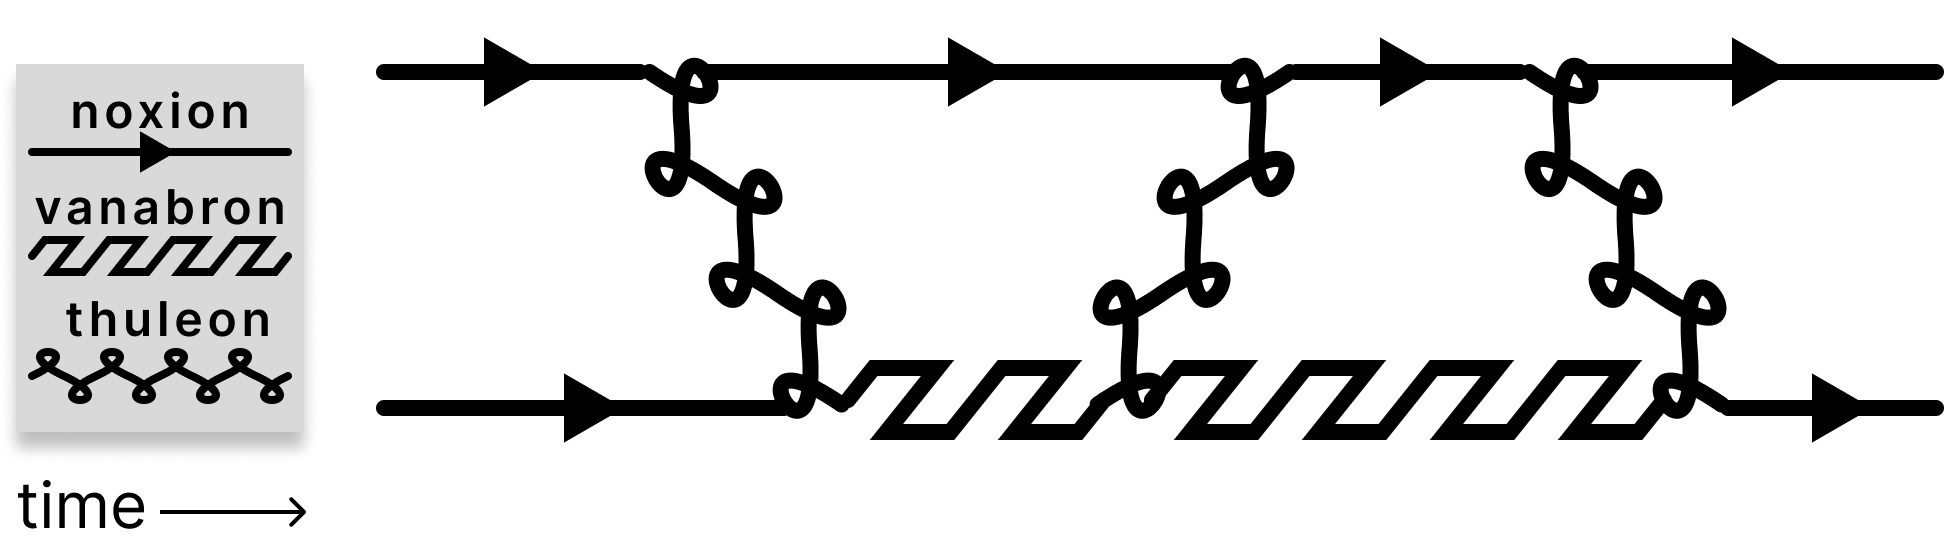
\includegraphics[width=0.8\textwidth]{tenebrivity/bw-complex-interaction.png}
  \end{center}
  While you know the tenebridges of the external particles (\(n_c + n_v \rightarrow n_c + n_v\)), you want to figure out how tenebridge conservation is maintained across all the inner interactions. First you associate each tenebridgial with a color to diagram:
  \begin{center}
    \vclr{vortex}, \cclr{crystal}, \fclr{flow}, and \sclr{spark}
  \end{center}
  Then, knowing the number of tenebridgials carried by each particle, you can then trace out the paths of the tenebridgials as they're exchanged by particles:
  \begin{center}
    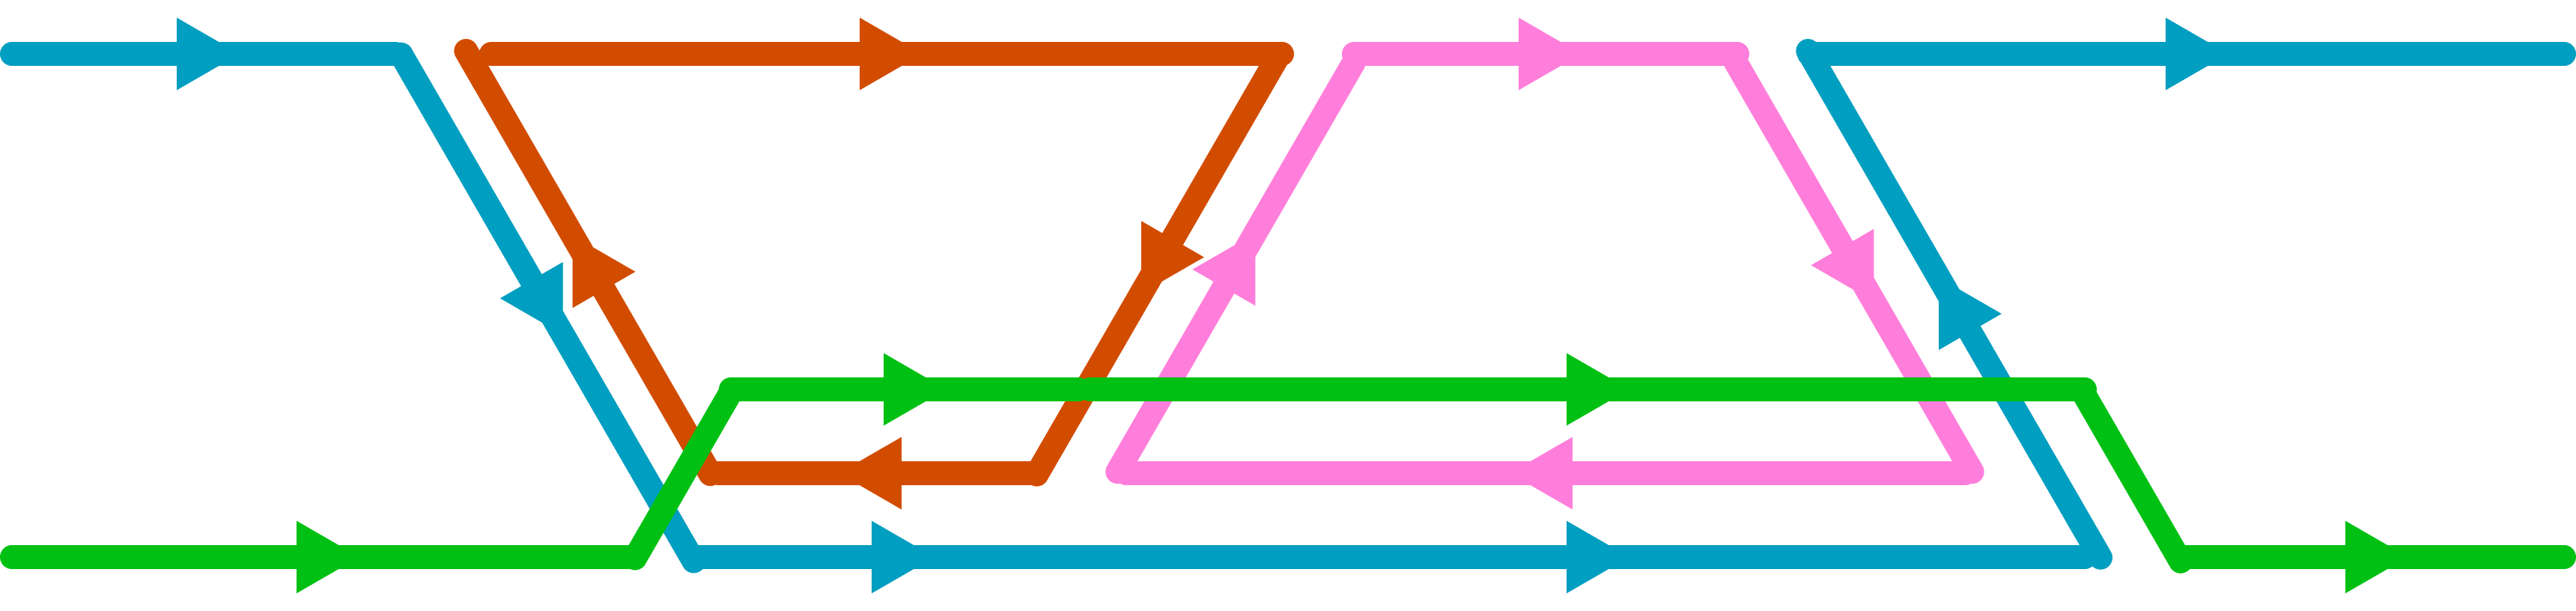
\includegraphics[width=0.8\textwidth]{tenebrivity/cl-complex-interaction.png}
  \end{center}
  One thing you might notice is that internally, the flow and spark tenebridgials are exchanged forward and then backward in time, effectively forming their own local time loops. This will behavior will become crucial in the understanding of contraparadoxical technologies.
\end{example}

\section{Field Theory}
To get started constructing our field theory, we need to establish the field representation of each particle, and the end goal is to build up the Lagrangian \(\mathcal{L}_{\text{QTD}}\), which can derive the dynamics of our fields by considering the energy terms associated with each particle and their interactions. This is no small feat; this section will simply present the solutions, as a full derivation would go well beyond this introductory review.

\subsection{Noxion Field}
Let's start with building the field representation of the noxion. Since we know the noxion is a spin-1/2 particle, it will behave as a Dirac spinor. Additionally, we need to represent any linear combination of the four tenebridgials; let's do this by defining \(\Psi\) to denote an arbitrary linear combination of tenebridgials:
\begin{definition}[Noxion Field Basis]
  \[\Psi_{\alpha} = \tau_1 \Psi_1 + \tau_2 \Psi_2 + \tau_3 \Psi_3 + \tau_4 \Psi_4 \equiv
    \begin{pmatrix}\tau_1 \\ \tau_2 \\ \tau_3 \\ \tau_4 \end{pmatrix}\]
  where \(\alpha\) runs from 1 to 4 to index the tenebridgial in the array \(\left[v, c, f, s \right]\).
\end{definition}

A tenebridge rotation can be expressed compactly by the action of an SU(4) matrix \(\sufour\) on the spinor \(\Psi\):
\[
  \Psi_{\alpha} \rightarrow \sufour_{\alpha\beta} \Psi_{\beta}
\]

\begin{definition}[SU(4) Basis]
  Any SU(4) matrix can be described as a linear combination of the 15 basis matrices; by convention these are defined as:\\
  \begin{center}

    \(\Omega^1 =
    \scriptscriptstyle \begin{pmatrix}
      \fourrow{0}{1}{0}{0} \\
      \fourrow{1}{0}{0}{0} \\
      \fourrow{0}{0}{0}{0} \\
      \fourrow{0}{0}{0}{0}
    \end{pmatrix}
    \),\,\,
    \(\Omega^2 =
    \scriptscriptstyle\begin{pmatrix}
      \fourrow{0}{-i}{0}{0} \\
      \fourrow{i}{0}{0}{0}  \\
      \fourrow{0}{0}{0}{0}  \\
      \fourrow{0}{0}{0}{0}
    \end{pmatrix}
    \),\,\,
    \(\Omega^3 =
    \scriptscriptstyle\begin{pmatrix}
      \fourrow{1}{0}{0}{0}  \\
      \fourrow{0}{-1}{0}{0} \\
      \fourrow{0}{0}{0}{0}  \\
      \fourrow{0}{0}{0}{0}
    \end{pmatrix}
    \),\,\,
    \(\Omega^4 =
    \scriptscriptstyle\begin{pmatrix}
      \fourrow{0}{0}{1}{0} \\
      \fourrow{0}{0}{0}{0} \\
      \fourrow{1}{0}{0}{0} \\
      \fourrow{0}{0}{0}{0}
    \end{pmatrix}
    \),\,\,
    \(\Omega^5 =
    \scriptscriptstyle\begin{pmatrix}
      \fourrow{0}{0}{-i}{0} \\
      \fourrow{0}{0}{0}{0}  \\
      \fourrow{i}{0}{0}{0}  \\
      \fourrow{0}{0}{0}{0}
    \end{pmatrix}
    \),\,\,
    \(\Omega^6 =
    \scriptscriptstyle\begin{pmatrix}
      \fourrow{0}{0}{0}{0} \\
      \fourrow{0}{0}{1}{0} \\
      \fourrow{0}{1}{0}{0} \\
      \fourrow{0}{0}{0}{0}
    \end{pmatrix}
    \),\,\,
    \(\Omega^7 =
    \scriptscriptstyle\begin{pmatrix}
      \fourrow{0}{0}{0}{0}  \\
      \fourrow{0}{0}{-i}{0} \\
      \fourrow{0}{i}{0}{0}  \\
      \fourrow{0}{0}{0}{0}
    \end{pmatrix}
    \),\,\,
    \(\Omega^8 = \nsqrt{3}
    \scriptscriptstyle\begin{pmatrix}
      \fourrow{1}{0}{0}{0}  \\
      \fourrow{0}{1}{0}{0}  \\
      \fourrow{0}{0}{-2}{0} \\
      \fourrow{0}{0}{0}{0}
    \end{pmatrix}
    \),\,\,
    \(\Omega^9 =
    \scriptscriptstyle\begin{pmatrix}
      \fourrow{0}{0}{0}{1} \\
      \fourrow{0}{0}{0}{0} \\
      \fourrow{0}{0}{0}{0} \\
      \fourrow{1}{0}{0}{0}
    \end{pmatrix}
    \),\,\,
    \(\Omega^{10} =
    \scriptscriptstyle\begin{pmatrix}
      \fourrow{0}{0}{0}{-i} \\
      \fourrow{0}{0}{0}{0}  \\
      \fourrow{0}{0}{0}{0}  \\
      \fourrow{i}{0}{0}{0}
    \end{pmatrix}
    \),\,\,
    \(\Omega^{11} =
    \scriptscriptstyle\begin{pmatrix}
      \fourrow{0}{0}{0}{0} \\
      \fourrow{0}{0}{0}{1} \\
      \fourrow{0}{0}{0}{0} \\
      \fourrow{0}{1}{0}{0}
    \end{pmatrix}
    \),\,\,
    \(\Omega^{12} =
    \scriptscriptstyle\begin{pmatrix}
      \fourrow{0}{0}{0}{0}  \\
      \fourrow{0}{0}{0}{-i} \\
      \fourrow{0}{0}{0}{0}  \\
      \fourrow{0}{i}{0}{0}
    \end{pmatrix}
    \),\,\,
    \(\Omega^{13} =
    \scriptscriptstyle\begin{pmatrix}
      \fourrow{0}{0}{0}{0} \\
      \fourrow{0}{0}{0}{0} \\
      \fourrow{0}{0}{0}{1} \\
      \fourrow{0}{0}{1}{0}
    \end{pmatrix}
    \),\,\,
    \(\Omega^{14} =
    \scriptscriptstyle\begin{pmatrix}
      \fourrow{0}{0}{0}{0}  \\
      \fourrow{0}{0}{0}{0}  \\
      \fourrow{0}{0}{0}{-i} \\
      \fourrow{0}{0}{i}{0}
    \end{pmatrix}
    \),\,\,
    \(\Omega^{15} = \nsqrt{6}
    \scriptscriptstyle\begin{pmatrix}
      \fourrow{1}{0}{0}{0} \\
      \fourrow{0}{1}{0}{0} \\
      \fourrow{0}{0}{1}{0} \\
      \fourrow{0}{0}{0}{-3}
    \end{pmatrix}
    \)
  \end{center}

  Since any general SU(4) matrix can be written as a combination of these, we can write the general form as:
  \[\sufour = \exp(i \phi^a\Omega^{a})\]
  Where the index \(a\) run from 1 to 15.\footnote{Recall that repeated indices indicate a summation; \(\phi^a\Omega^{a} \equiv \sum^{15}_{a=1}\phi^a\Omega^{a} \) }
\end{definition}

In the scenario where two people are making tenebridge measurements, there is no guarantee that they are using the same basis. Relativity adds the restriction that two bases at different locations instantaneously. Therefore, the SU(4) transformations depend on the position four-vector \(x\),:
\[\sufour(x) = \phi^a(x) \sufour^a\]

This presents a slight problem. Our end goal is to build the Lagrangian, and the most basic kinetic term would look something like:
\[
  \mathcal{L}_{\text{noxion}} = \bar{\Psi} i \gamma \partial \Psi
\]
However, looking at an SU(4) transformation happening on this term, the derivative now acts on our SU(4) matrices, so for an SU(4) rotation on this term:
\begin{align*}
  \mathcal{L}_{\text{noxion}} = \bar{\Psi} i \gamma \partial \Psi
  \longrightarrow \mathcal{L}^{\mathfrak{su}(4)}_{\text{noxion}}
   & = \bar{\Psi} \sufour^{\dag} i \gamma \partial \sufour \Psi                               \\
   & = \bar{\Psi} i \gamma \partial \Psi  - \bar{\Psi}\Omega^{a}\gamma\partial \phi^a(x) \Psi \\
   & = \mathcal{L}_{\text{noxion}} - \bar{\Psi}\Omega^{a}\gamma\partial \phi^a(x) \Psi
\end{align*}
we see that this Lagrangian is no longer invariant under an SU(4) transformation. In order to restore this symmetry to conserve tenebridge, we \textit{must} introduce a new field that transforms in a way to cancel out the leftover term. We'll label this field \(V^a\), to cancel out the leftover term and derive the following:
\[
  \mathcal{L}_{\text{noxion}} + \mathcal{L}_{?} = \bar{\Psi} i \gamma \partial \Psi + g\bar{\Psi}\gamma V^{a} \Omega^{a} \Psi
\]
Now let's consider the term we've just added. \(a\) runs from 1 to 15, so our \(V^a\) field must also have 15 types to match. What is this mysterious \(V^a\)? Well, it turns out to be the vanibron field! Take a moment to interpret this - in order for noxions to conserve tenebridge, they \textit{must} be able to interact with a vanibron field. In short, this is the field tenebridge conservation analogous to this particle tenebridge conservation:
\begin{center}
  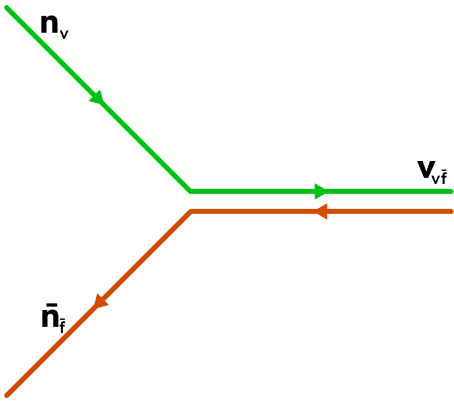
\includegraphics[width=0.3\textwidth]{tenebrivity/cl-nvn.png}
\end{center}
That is to say, tenebridge conservation is maintained when vanibrons have a tenebridgial-antitenebridgial pair equivalent to two noxions with different tenebridges. This also means that the term we've added is in fact the \(\mathcal{L}_{\text{nox-van-nox}}\), the Lagrangian for the interaction between noxions and vanibrons.

\section{Vanibron Field}
So far we've described the vanibron field as a family of \(V^a\) fields, with \(a\) running from 1 to 15. You may be wondering - if there are 4 tenebridgials and vanibrons can carry two at a time, then shouldn't there be \textit{16} fields for each combination
\[
  \begin{matrix}
    v\bar{v} & v\bar{c} & v\bar{f} & v\bar{s} \\
    c\bar{v} & c\bar{c} & c\bar{f} & c\bar{s} \\
    f\bar{v} & f\bar{c} & f\bar{f} & f\bar{s} \\
    s\bar{v} & s\bar{c} & s\bar{f} & s\bar{s} \\
  \end{matrix}\qquad?
\]
Well as we saw before, vanibrons can only have a tenebridge derived from two noxions. Those two noxions \textit{must} have differing tenebridgials, because if they were the same, then it would be impossible to exchange and also conserve tenebridge:
\begin{center}
  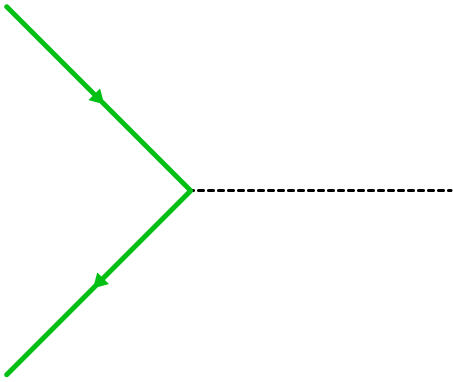
\includegraphics[width=0.3\textwidth]{tenebrivity/xlb-cl-nxn.png}
\end{center}
This means the ``singlet'' states -- \(v\bar{v}\), \(c\bar{c}\), \(f\bar{f}\), and \(s\bar{s}\) -- are not allowed. You may ask, but then doesn't that mean there are only 12 states? Well keep in mind that this is a \textit{quantum} theory, meaning a superposition can be made out of any combination of states. Therefore, there is truly only \textit{one} invalid state - the state in which a vanibron could be measured and seen in \textit{any} singlet state:
\[
  \left( v\bar{v} + c\bar{c} + f\bar{f} + s\bar{s} \right)/2
\]
Ensuring this state is unreachable, we want to then develop a basis that still gives otherwise a linearly independent set of 15 states. Fortunately, we already have this set - the \(\Omega\) matrices! Therefore, the basis we use for the vanibrons is:
\begin{definition}[Vanibron Field Basis]
  \[V^a = \begin{pmatrix}
      v\bar{v} & v\bar{c} & v\bar{f} & v\bar{s} \\
      c\bar{v} & c\bar{c} & c\bar{f} & c\bar{s} \\
      f\bar{v} & f\bar{c} & f\bar{f} & f\bar{s} \\
      s\bar{v} & s\bar{c} & s\bar{f} & s\bar{s} \\
    \end{pmatrix}_{ij} \Omega^a_{ij}  \]
\end{definition}

Fully expanded, the 15 states are:
\[
  \begin{array}{cccc}
    V^1=\frac{v \bar{c}+c \bar{v}}{\sqrt{2}}                 & V^2=-\frac{i \left(v \bar{c}-c \bar{v}\right)}{\sqrt{2}}    & V^3=\frac{v \bar{v}-c \bar{c}}{\sqrt{2}}                            & V^4=\frac{v \bar{f}+f \bar{v}}{\sqrt{2}}                   \\
    V^5=-\frac{i \left(v \bar{f}-f \bar{v}\right)}{\sqrt{2}} & V^6=\frac{f \bar{c}+c \bar{f}}{\sqrt{2}}                    & V^7=\frac{i \left(f \bar{c}-c \bar{f}\right)}{\sqrt{2}}             & V^8=\frac{c \bar{c}-2 f \bar{f}+v \bar{v}}{\sqrt{6}}       \\
    V^9=\frac{v \bar{s}+s \bar{v}}{\sqrt{2}}                 & V^{10}=-\frac{i \left(v \bar{s}-s \bar{v}\right)}{\sqrt{2}} & V^{11}=\frac{s \bar{c}+c \bar{s}}{\sqrt{2}}                         & V^{12}=\frac{i \left(s \bar{c}-c \bar{s}\right)}{\sqrt{2}} \\
    V^{13}=\frac{s \bar{f}+f \bar{s}}{\sqrt{2}}              & V^{14}=\frac{i \left(s \bar{f}-f \bar{s}\right)}{\sqrt{2}}  & V^{15}=\frac{c \bar{c}+f \bar{f}-3 s \bar{s}+v \bar{v}}{2 \sqrt{3}} & \text{}                                                    \\
  \end{array}
\]
This basis ensures that no singlet state can be formed and still recreate all the known tenebridgial combinations:
\[
  \begin{array}{cccc}
    v\bar{c} = \frac{V^1+iV^2}{\sqrt{2}}
     & c\bar{v} = \frac{V^1-iV^2}{\sqrt{2}}
     & v\bar{f} = \frac{V^4+iV^5}{\sqrt{2}}
     & f\bar{v} = \frac{V^4-iV^5}{\sqrt{2}}       \\
    v\bar{s} = \frac{V^9+iV^{10}}{\sqrt{2}}
     & s\bar{v} = \frac{V^{9}-iV^{10}}{\sqrt{2}}
     & c\bar{f} = \frac{V^{6}+iV^{7}}{\sqrt{2}}
     & f\bar{c} = \frac{V^{6}-iV^{7}}{\sqrt{2}}   \\
    c\bar{s} = \frac{V^{11}+iV^{12}}{\sqrt{2}}
     & s\bar{c} = \frac{V^{11}-iV^{12}}{\sqrt{2}}
     & f\bar{s} = \frac{V^{13}+iV^{14}}{\sqrt{2}}
     & s\bar{f} = \frac{V^{13}-iV^{14}}{\sqrt{2}}
  \end{array}
\]

One thing to watch out for however is that vanibrons are spin-1 particles, meaning that their field is a \textbf{four-vector field}. For example, you might use the definition above to write the explicit form of the 1st vanibron state, but the terms in that result are four-vectors:
\[
  V^1 = i(c\bar{v}-v\bar{c}) = i\fourvec{%
    V^1_0(\mathbf{x})%
  }{
    V^1_1(\mathbf{x})
  }{
    V^1_2(\mathbf{x})
  }{
    V^1_3(\mathbf{x})
  }
\]
If we are working with this field in a context where we need to consider spacetime transformations, then its sometimes helpful to fully index the field as
\[
  V^a_{\mu}(\mathbf{x}) = \fourvec{%
    V^a_0(\mathbf{x})%
  }{
    V^a_1(\mathbf{x})
  }{
    V^a_2(\mathbf{x})
  }{
    V^a_3(\mathbf{x})
  }
\]

Since this is a vector field, the kinetic term of the Lagrangian isn't just a simple multivariable derivative -- we need to capture the derivative of each component in each direction. To do so, we would normally define a Field Strength Tensor

\[\mho^a_{\mu \nu} \overset{?}{=} \partial_{\mu}V^a_{\nu} - \partial_{\nu}V^a_{\mu}\]

and this would lead to a Lagrangian like

\[
  \mathcal{L}_{\text{vanibron}} = -\frac{1}{4} \mho^a_{\mu \nu} \mho^{a \mu \nu}.
\]

Does this Lagrangian still follow SU(4) gauge invariance? First let's check how the vanibron field transforms:
\[
  V^a_{\mu} \rightarrow V^{\prime a}_{\mu} \sufour V^a_{\mu} \sufour^{\dag} + \frac{i}{g_v} \sufour \partial_{\mu} \sufour^{\dag}
\]

Recalling the original definition \(\sufour = \exp(i \phi^a \Omega^a)\) and considering only first order terms in \(\phi^a\), the change \(\delta V^a_{\mu}\) due to the gauge transformation is:
\[
  \delta V^a_{\mu} = V^{\prime a}_{\mu} - V^a_{\mu} \approx i \phi^b\left(\Omega^b V^{\prime a}_{\mu} - V^{\prime a}_{\mu}\Omega^b \right) + \frac{i}{g_v} \partial_{\mu} \phi^b \Omega^b
\]

The term \(\Omega^b V^{\prime a}_{\mu} - V^{\prime a}_{\mu}\Omega^b\) doesn't vanish as the SU(4) generators do not commute. Instead, we can use the non-commutative property of the SU(4) generators:
\[
  \Omega^a\Omega^b -  \Omega^b\Omega^a = i \omega^{abc}\Omega^c
\]
where \(\omega^{abc}\) are referred to as the SU(4) structure constants. Using this, we can write the vanibron field change as:
\[
  \delta V^a_{\mu} \approx \omega^{abc}\phi^bV^c_{\mu} + \frac{i}{g_v} \partial_{\mu} \phi^b \Omega^b
\]
Now finally let's see how the field strength tensor \(\Phi^a_{\mu\nu}\) transforms; looking specifically at the change due to the gauge transformation:
\begin{align*}
  \delta\mho^a_{\mu \nu}
   & = \partial_{\mu}\delta V^a_{\nu} - \partial_{\nu}\delta V^a_{\mu}                        \\
   & \approx \omega^{abc}\phi^b\left(\partial_{\mu}V^c_{\nu} - \partial_{\nu}V^c_{\mu}\right)
  +\omega^{abc}V^c_{\mu}\partial_{\nu}\phi^b - \omega^{abc}V^c_{\nu}\partial_{\mu}\phi^b
\end{align*}
The last two terms contain products of \(V^c_{\mu}\) and derivatives of \(\phi^b\). These terms aren't canceled by any term in our naive definition of \(\mho^a_{\mu \nu}\). In order to counteract those terms then, we must update our definition to introduce a new term:
\begin{definition}[Vanibron Field Strength Tensor]
  \[\mho^a_{\mu \nu} \equiv \partial{\mu}V^a_{\nu} - \partial{\nu}V^a_{\mu} + g_v \omega^{abc}V^{b}_{\mu}V^{c}_{\nu} \]
\end{definition}

Our Lagrangian then can be written correctly as:
\[
  \mathcal{L}_{\text{vanibron}} = -\frac{1}{4} \mho^a_{\mu \nu} \mho^{a \mu \nu}
\]

Let's take a moment to interpret our results. The Lagrangian now contains terms of order \(\mho^3\) and \(\mho^4\) - in fact these are the vanibron's \textit{self} interactions! Just as the noxion can experience the tenebrivic force mediated by a vanibron, so can the vanibron experience the tenebrivic force mediated by a vanibron!
\begin{center}
  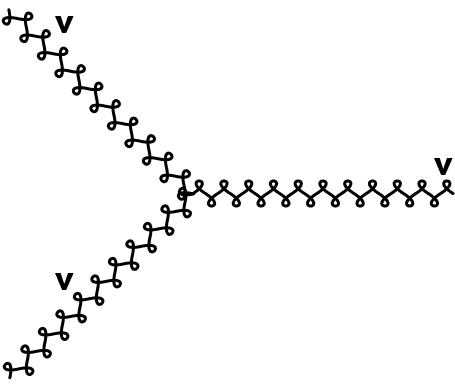
\includegraphics[width=0.3\textwidth]{tenebrivity/bw-v3.png}
  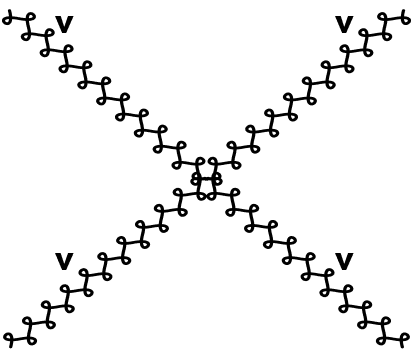
\includegraphics[width=0.3\textwidth]{tenebrivity/bw-v4.png}
\end{center}
Tenebridge is still conserved in these interactions as well, which we can see by tracing out the paths of tenebridge exchange in these interactions:
\begin{center}
  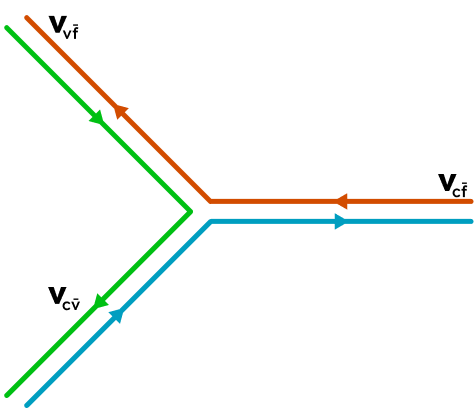
\includegraphics[width=0.3\textwidth]{tenebrivity/cl-v3.png}
  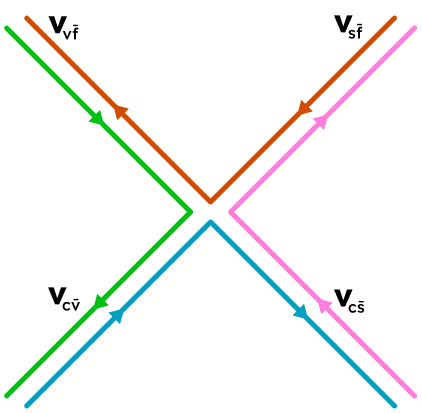
\includegraphics[width=0.3\textwidth]{tenebrivity/cl-v4.png}
\end{center}

\section{Thuleon Field}

The thuleon is another particle that carries tenebridge and experiences tenebrivity mediated by the vanibron. It is a spin-\(\frac{3}{2}\) particle, and also has mass, so in its rest frame there are four helicity states: \(\pm\frac{3}{2}\) and \(\pm\frac{1}{2}\).

The next attribute of the thuleon to account for is its tenebridge. Thuleons carry three tenebridgials at a time, and there are four possible ways to do so:
\[\left\{cfv,fsv,csv,cfs\right\}\]
Order isn't distinct for these combinations (e.g.\ cfv and vfc would refer to the same combination), but there is one other factor to account for stemming from tenebridge conservation. Take a look at the interactions involving thuleons:
\begin{center}
  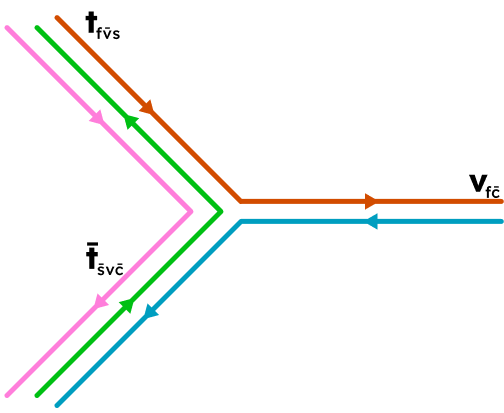
\includegraphics[width=0.3\textwidth]{tenebrivity/cl-tvt.png}
  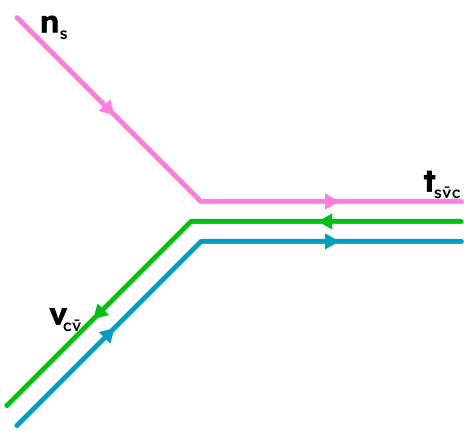
\includegraphics[width=0.3\textwidth]{tenebrivity/cl-nvt.png}
\end{center}

In both cases, the thuleon has a distinct signature of tenebridgial-antitenebridgial-tenebridgial. This means for each combination, it is possible to distinguish by which of the three tenebridgials is in the "anti" slot. For example, \(c\bar{f}v\) and \(cf\bar{v}\) are distinguishable states, but \(c\bar{f}v\) and \(v\bar{f}c\) are not.

Finally, because the particle is spin-\(\frac{3}{2}\), it must take on the form of a vector-spinor field.

\begin{definition}[Thuleon Field Representation]
  To incorporate all of the above, we will need 4 indices:
  \begin{enumerate}
    \item an index \(\eta\) ranging from 0 to 3\\
          for the given helicity state \(\left\{\frac{3}{2},\frac{1}{2},-\frac{1}{2},-\frac{3}{2}\right\}\)
    \item an index \(\mu\) ranging from 0 to 3\\
          for the components of the vector field in the \(\mu\)-th dimension
    \item an index \(\tau\) ranging from 0 to 3\\
          for the standard tenebridgial ordering \(\left\{v,c,f,s\right\}\),\\
          the index represents which tenebridgial is missing in the combination:
          \(\left\{cfs,vfs,vcs,vcf\right\}\)
    \item an index \(\chi\) ranging from 1 to 3\\
          for which tenebridgial in the combination is the antitenebridgial.\\
          e.g.\ for \(\tau=0\), \(\chi\) ranges over \(\left\{\bar{c}fs,c\bar{f}s,cf\bar{s}\right\}\)
  \end{enumerate}
  Then we can define the thuleon field as a \(4\times4\times4\times3\) tensor:
  \begin{equation}
    \Theta^{\eta}_{\mu \tau \chi}
    =
    \begin{pmatrix}s_{3/2}\\s_{1/2}\\s_{-1/2}\\s_{-3/2}\end{pmatrix}_{\eta}
    \begin{pmatrix}
      \left(t_{f \bar{c} s}\right)_{\mu} & \left(t_{c \bar{f} s}\right)_{\mu} & \left(t_{c \bar{s} f}\right)_{\mu} \\
      \left(t_{f \bar{v} s}\right)_{\mu} & \left(t_{v \bar{f} s}\right)_{\mu} & \left(t_{v \bar{s} f}\right)_{\mu} \\
      \left(t_{c \bar{v} s}\right)_{\mu} & \left(t_{v \bar{c} s}\right)_{\mu} & \left(t_{v \bar{s} c}\right)_{\mu} \\
      \left(t_{c \bar{v} f}\right)_{\mu} & \left(t_{v \bar{c} f}\right)_{\mu} & \left(t_{v \bar{f} c}\right)_{\mu}
    \end{pmatrix}_{\tau \chi}
  \end{equation}
  The first matrix contains the spinor portion of this field, while the second contains the vector portion of this field, so we have indeed constructed a spinor-vector field as necessary for a spin-\(\frac{3}{2}\) particle.
\end{definition}

In a relativistic theory, normally the presence of the antiparticle would double the number of distinguishable states, but later we will see that the negative mass of the antithuleon enforces that the antithuleon is its own adjoint, so instead of a single \(\Theta\) vector-spinor field with components for both the particle and antiparticle, instead \(\Theta\) represents all the components for the thuleon and \(\bar{\Theta}\) will represent all the components for the antithuleon. This does have a specific interpretation: the thuleon isn't quite its own antiparticle, but rather, the ``spin \(\eta\), \(a\) -- anti-\(b\) -- \(c\) thuleon'' is indistinguishable from the ``spin \(-\eta\), anti-\(a\) -- \(b\) -- anti-\(c\) antithuleon of same mass''. Explicitly, this means the adjoint of the field looks like:
\[
  \bar{\Theta}^{\eta}_{\mu \tau \chi}
  =
  \begin{pmatrix}s_{-3/2}\\s_{-1/2}\\s_{1/2}\\s_{3/2}\end{pmatrix}_{\eta}
  \begin{pmatrix}
    \left(\bar{t}_{\bar{f} c \bar{s}}\right)_{\mu} & \left(\bar{t}_{\bar{c} f \bar{s}}\right)_{\mu} & \left(\bar{t}_{\bar{c} s \bar{f}}\right)_{\mu} \\
    \left(\bar{t}_{\bar{f} v \bar{s}}\right)_{\mu} & \left(\bar{t}_{\bar{v} f \bar{s}}\right)_{\mu} & \left(\bar{t}_{\bar{v} s \bar{f}}\right)_{\mu} \\
    \left(\bar{t}_{\bar{c} v \bar{s}}\right)_{\mu} & \left(\bar{t}_{\bar{v} c \bar{s}}\right)_{\mu} & \left(\bar{t}_{\bar{v} s \bar{c}}\right)_{\mu} \\
    \left(\bar{t}_{\bar{c} v \bar{f}}\right)_{\mu} & \left(\bar{t}_{\bar{v} c \bar{f}}\right)_{\mu} & \left(\bar{t}_{\bar{v} f \bar{c}}\right)_{\mu} \\
  \end{pmatrix}_{\tau \chi}
\]

\subsection{Kinetic Term}

The kinetic term of this Lagrangian can be derived much the same way as both the noxion's and vanibron's, where the spinor portion of the thuleon follows the noxion's derivation and the vector portion of the thuleon follows the vanibron's derivation.

Let's define a field strength tensor for the vector portion of the field:
\begin{definition}[Thuleon Field Strength Tensor]
  \[
    \mathfrak{T}^{\eta}_{\mu \nu ; \tau \chi} = \partial_{\mu}\Theta^{\eta}_{\nu \tau \chi} - \partial_{\nu}\Theta^{\eta}_{\mu \tau \chi}
  \]
\end{definition}

Following the same derivation of the Lagrangian by gauge invariance leads us to a free-particle Lagrangian which we can compose in two parts; the kinetic contribution from the tensor and spinor:
\[
  \mathcal{L}_{\text{thuleon}} = -\frac{1}{4}\mathfrak{T}^{\eta}_{\mu \nu ; \tau \chi}\gamma^{\eta} \mathfrak{T}^{\eta \mu \nu}_{ \tau \chi}
\]

and the gauge-invariance requirement that leads to the vanibron-interaction term:
\[
  \mathcal{L}_{\text{thu-van}} \overset{?}{=} - i g_{\eth} \bar{\Theta}^{\eta}_{\tau \chi} \gamma^{\mu}  \Omega^a V^a_{\mu}  \bar{\Theta}^{\eta}_{\tau \chi}
\]
except there's a problem with that Lagrangian as written.

\subsection{Thuleon-Vanibron Interaction}
\begin{center}
  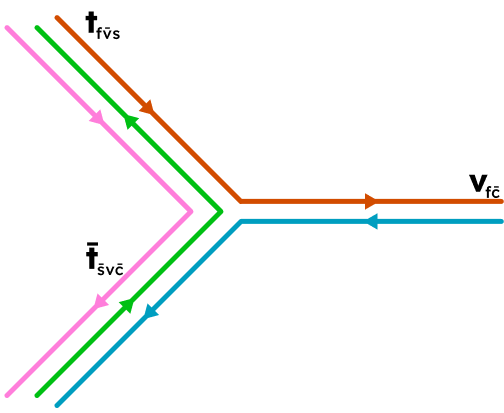
\includegraphics[width=0.3\textwidth]{tenebrivity/cl-tvt.png}
\end{center}
Not every kind of thuleon can interact with every kind of vanibron, since tenebridge conservation requires \(t_{a\bar{b}c} \rightarrow t_{a\bar{b}d} + v_{c\bar{d}} \). Therefore, the thuleon-vanibron interaction term requires an additional factor to enforce this coupling. First let's think through an example:
\begin{example}[Thuleon Mapping]
  \(\Theta^{\eta}_{01}\) is an \(\bar{c}fv\) thuleon. Tenebridge is conserved if the resulting particles are an \(f\bar{c}s\) thuleon and \(v\bar{s}\) vanibron, or \(s\bar{c}v\) thuleon and \(f\bar{s}\) vanibron.
  \begin{itemize}
    \item In the former case, the associated fields are \(\Theta^{\eta}_{3,3}\) and \(\nsqrt{2}\left(V^9 - i V^{10}\right)\)
    \item In the latter case, the associated fields are \(\Theta^{\eta}_{2,1}\) and \(\nsqrt{2}\left(V^{13} - i V^{14}\right)\)
  \end{itemize}
\end{example}

\newcommand{\tvtmat}{\ensuremath{\aleph_a^{\tau \chi \lambda \rho}}}

Thinking through each case of the example above, we see that the vanibron interaction term will require a transformation matrix \(\tvtmat\) in order to restrict the coupling accordingly:
\[
  - i g_{\eth}
  \bar{\Theta}^{\eta}_{\mu \lambda \rho}
  \gamma^{\mu}
  \tvtmat
  \Omega^a
  V^a_{\mu}
  \bar{\Theta}^{\eta}_{\mu \tau \chi}
\]



To find the explict form of \(\tvtmat\), we consider each possible interaction
\begin{align*}
   & \begin{Bmatrix}
       t_{f \bar{c} s} & t_{c \bar{f} s} & t_{c \bar{s} f} \\
       t_{f \bar{v} s} & t_{v \bar{f} s} & t_{v \bar{s} f} \\
       t_{c \bar{v} s} & t_{v \bar{c} s} & t_{v \bar{s} c} \\
       t_{c \bar{v} f} & t_{v \bar{c} f} & t_{v \bar{f} c}
     \end{Bmatrix}                                        \\
   & \longrightarrow
  \begin{Bmatrix}
    t_{v \bar{c} s}+v_{f \bar{v}} & t_{v \bar{f} s}+v_{c \bar{v}} & t_{v \bar{s} f}+v_{c \bar{v}} \\
    t_{c \bar{v} s}+v_{f \bar{c}} & t_{c \bar{f} s}+v_{v \bar{c}} & t_{c \bar{s} f}+v_{v \bar{c}} \\
    t_{f \bar{v} s}+v_{c \bar{f}} & t_{f \bar{c} s}+v_{v \bar{f}} & t_{f \bar{s} c}+v_{v \bar{f}} \\
    t_{s \bar{v} f}+v_{c \bar{s}} & t_{s \bar{c} f}+v_{v \bar{s}} & t_{s \bar{f} c}+v_{v \bar{s}} \\
  \end{Bmatrix} \\
   & \lor
  \begin{Bmatrix}
    t_{f \bar{c} v}+v_{s \bar{v}} & t_{c \bar{f} v}+v_{s \bar{v}} & t_{c \bar{s} v}+v_{f \bar{v}} \\
    t_{f \bar{v} c}+v_{s \bar{c}} & t_{v \bar{f} c}+v_{s \bar{c}} & t_{v \bar{s} c}+v_{f \bar{c}} \\
    t_{c \bar{v} f}+v_{s \bar{f}} & t_{v \bar{c} f}+v_{s \bar{f}} & t_{v \bar{s} f}+v_{c \bar{f}} \\
    t_{c \bar{v} s}+v_{f \bar{s}} & t_{v \bar{c} s}+v_{f \bar{s}} & t_{v \bar{f} s}+v_{c \bar{s}} \\
  \end{Bmatrix}
\end{align*}
then map these to the appropriate field
\begin{align*}
   & \begin{Bmatrix}
       \Theta _{\mu,0,1}^{\eta} & \Theta _{\mu,0,2}^{\eta} & \Theta _{\mu,0,3}^{\eta} \\
       \Theta _{\mu,1,1}^{\eta} & \Theta _{\mu,1,2}^{\eta} & \Theta _{\mu,1,3}^{\eta} \\
       \Theta _{\mu,2,1}^{\eta} & \Theta _{\mu,2,2}^{\eta} & \Theta _{\mu,2,3}^{\eta} \\
       \Theta _{\mu,3,1}^{\eta} & \Theta _{\mu,3,2}^{\eta} & \Theta _{\mu,3,3}^{\eta}
     \end{Bmatrix} \\
   & \longrightarrow
  \begin{Bmatrix}
    \Theta _{\mu,2,2}+\vanfv & \Theta _{\mu,1,2}+\vancv & \Theta _{\mu,1,3}+\vancv \\
    \Theta _{\mu,3,1}+\vanfc & \Theta _{\mu,0,2}+\vanvc & \Theta _{\mu,0,3}+\vanvc \\
    \Theta _{\mu,1,1}+\vancf & \Theta _{\mu,0,0}+\vanvf & \Theta _{\mu,0,3}+\vanvf \\
    \Theta _{\mu,1,1}+\vancs & \Theta _{\mu,0,0}+\vanvs & \Theta _{\mu,0,2}+\vanvs \\
  \end{Bmatrix}    \\
   & \lor
  \begin{Bmatrix}
    \Theta _{\mu,3,0}+\vansv & \Theta _{\mu,3,3}+\vansv & \Theta _{\mu,2,3}+\vanfv \\
    \Theta _{\mu,3,1}+\vansc & \Theta _{\mu,3,2}+\vansc & \Theta _{\mu,2,3}+\vanfc \\
    \Theta _{\mu,3,1}+\vansf & \Theta _{\mu,3,2}+\vansf & \Theta _{\mu,1,2}+\vancf \\
    \Theta _{\mu,2,1}+\vanfs & \Theta _{\mu,2,2}+\vanfs & \Theta _{\mu,1,2}+\vancs \\
  \end{Bmatrix}
\end{align*}
then the full form of \(\tvtmat\) can be formed by grabbing the indices from the above mapping:
\begin{align*}
  \aleph_a^{\tau \chi \lambda \rho}
   & =\alentry{0}{1}{2}{2}{4}{-}{5}{3}{0}{9}{-}{10} \\
   & +\alentry{0}{2}{1}{2}{1}{-}{2}{3}{3}{9}{-}{10} \\
   & +\alentry{0}{3}{1}{3}{1}{-}{2}{2}{3}{4}{-}{5}  \\
   & +\ldots
\end{align*}

\subsection{Thuleon-Vanibron-Noxion Interaction}
\begin{center}
  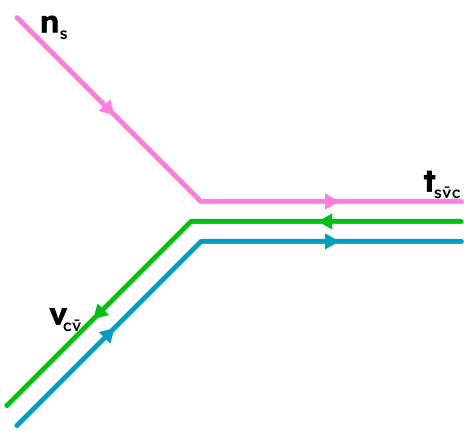
\includegraphics[width=0.3\textwidth]{tenebrivity/cl-nvt.png}
\end{center}
There's yet another interaction we have yet to account for, which is the interaction between a single noxion, vanibron, and thuleon. Such an interaction term might look like:
\[
  \beth^{a b c}_{d} \Upsilon_{\eta \kappa} \left(
  g_{tvn}
  \bar{\Theta}^{\eta}_{\mu a b}
  \gamma^{\eta}
  \Omega^{d}
  V^{d}_{\mu}
  \gamma^{\kappa}
  \Psi^{\kappa}_{c}
  +
  g_{nvt}
  \bar{\Psi}^{\kappa}_{c}
  \gamma^{\kappa}
  \Omega^{d}
  \bar{V}^{d}_{\mu}
  \gamma^{\eta}
  \Theta^{\eta}_{\mu a b}
  \right)
\]
where the two terms represent the forward and reverse process both being possible, with rates determined by the coupling constants \(g_{tvn}\) and \(g_{nvt}\). Tenebridge conservation leads to the \(\beth^{a b c}_{d}\) term to ensure that only valid transformations occur. This can be derived following the transformation rules:
\begin{align*}
   & \begin{Bmatrix}
       t_{f \bar{c} s} & t_{c \bar{f} s} & t_{c \bar{s} f} \\
       t_{f \bar{v} s} & t_{v \bar{f} s} & t_{v \bar{s} f} \\
       t_{c \bar{v} s} & t_{v \bar{c} s} & t_{v \bar{s} c} \\
       t_{c \bar{v} f} & t_{v \bar{c} f} & t_{v \bar{f} c}
     \end{Bmatrix} \\
   & \longrightarrow
  \begin{Bmatrix}
    n_{f} + v_{s \bar{c}} & n_{c} + v_{s \bar{f}} & n_{c} + v_{f \bar{s}} \\
    n_{f} + v_{s \bar{v}} & n_{v} + v_{s \bar{f}} & n_{v} + v_{f \bar{s}} \\
    n_{c} + v_{s \bar{v}} & n_{v} + v_{s \bar{c}} & n_{v} + v_{c \bar{s}} \\
    n_{c} + v_{f \bar{v}} & n_{v} + v_{f \bar{c}} & n_{v} + v_{c \bar{f}}
  \end{Bmatrix} \lor
  \begin{Bmatrix}
    n_{s} + v_{f \bar{c}} & n_{s} + v_{c \bar{f}} & n_{f} + v_{c \bar{s}} \\
    n_{s} + v_{f \bar{v}} & n_{s} + v_{v \bar{f}} & n_{f} + v_{v \bar{s}} \\
    n_{s} + v_{c \bar{v}} & n_{s} + v_{v \bar{c}} & n_{c} + v_{v \bar{s}} \\
    n_{f} + v_{c \bar{v}} & n_{f} + v_{v \bar{c}} & n_{c} + v_{v \bar{f}}
  \end{Bmatrix}
\end{align*}

and then considering the equivalent fields
\begin{align*}
   & \begin{Bmatrix}
       \Theta _{\mu,0,1}^{\eta} & \Theta _{\mu,0,2}^{\eta} & \Theta _{\mu,0,3}^{\eta} \\
       \Theta _{\mu,1,1}^{\eta} & \Theta _{\mu,1,2}^{\eta} & \Theta _{\mu,1,3}^{\eta} \\
       \Theta _{\mu,2,1}^{\eta} & \Theta _{\mu,2,2}^{\eta} & \Theta _{\mu,2,3}^{\eta} \\
       \Theta _{\mu,3,1}^{\eta} & \Theta _{\mu,3,2}^{\eta} & \Theta _{\mu,3,3}^{\eta}
     \end{Bmatrix} \\
   & \longrightarrow
  \begin{Bmatrix}
    n_{3} + \vansc & n_{2} + \vansf & n_{2} + \vanfs \\
    n_{3} + \vansv & n_{1} + \vansf & n_{1} + \vanfs \\
    n_{2} + \vansv & n_{1} + \vansc & n_{1} + \vancs \\
    n_{2} + \vanfv & n_{1} + \vanfc & n_{1} + \vancf
  \end{Bmatrix}                                  \\
   & \lor
  \begin{Bmatrix}
    n_{4} + \vanfc & n_{4} + \vancf & n_{3} + \vancs \\
    n_{4} + \vanfv & n_{4} + \vanvf & n_{3} + \vanvs \\
    n_{4} + \vancv & n_{4} + \vanvc & n_{2} + \vanvs \\
    n_{3} + \vancv & n_{3} + \vanvc & n_{2} + \vanvf
  \end{Bmatrix}
\end{align*}

Then the various entries of \(\beth^{a b c}_{d}\) can be derived as:
\begin{align*}
  \beth^{a b c}_{d}
   & = \nsqrt{2}\kron{a}{0}\kron{b}{1}\left(
  \kron{c}{3}\left(
    \kron{d}{11} - i\kron{d}{12}
    \right)+
  \kron{c}{4}\left(
    \kron{d}{6} - i\kron{d}{7}
    \right)
  \right)                                    \\
   & + \nsqrt{2}\kron{a}{0}\kron{b}{2}\left(
  \kron{c}{2}\left(
    \kron{d}{13} - i\kron{d}{14}
    \right)+
  \kron{c}{4}\left(
    \kron{d}{6} + i\kron{d}{7}
    \right)
  \right)                                    \\
   & + \nsqrt{2}\kron{a}{0}\kron{b}{3}\left(
  \kron{c}{2}\left(
    \kron{d}{13} + i\kron{d}{14}
    \right)+
  \kron{c}{3}\left(
    \kron{d}{11} + i\kron{d}{12}
    \right)
  \right)                                    \\
   & + \ldots
\end{align*}


\subsection{Mass Term}
The thuleon not only has mass, but infamously the antithuleon has negative mass. Writing the lagrangian contribution for this is actually relatively straightforward:
\begin{definition}[Thuleon Mass Lagrangian]
  \[
    \mathcal{L}_{\text{thuleon-mass}} \equiv \mathfrak{m} \left(
    \bar{\Theta}^{\eta}_{\tau \chi}\Theta^{\eta}_{\tau \chi} - \bar{\Theta}^{3-\eta}_{3-\tau,3-\chi}\Theta^{3-\eta}_{3-\tau,3-\chi}
    \right)
  \]
\end{definition}

The more interesting discussion is the impact that a particle with negative mass has on our understanding of the universe. Let's review what topics are impacted, or otherwise not impacted.

\subsubsection{Vacuum Stability}
Typically, the vacuum state in a quantum field theory is the lowest energy state. A negative mass term could create the possibility of a vacuum that is not the global energy minimum. Such a vacuum would be unstable and susceptible to decaying to a state of even lower energy. This can lead to a phenomenon called ``vacuum decay''.

In QTD, From the reference frame of the antithuleon, a vacuum decay would be seen as \textit{increasing} the energy state of the antithuleon. This is therefore an antithuleon excitation. Just as an electron excitation leads to photon emission as the electron returns to ground state, the antithuleon excitation drives the antithuleon to couple with a thuleon to decay into the massless vanibron. Therefore, local vacuum decay generally doesn't occur.

However, in the history of the universe, antithuleon-thuleon pairs could be separated by processes like thuleon Hawking radiation. In this case, the free antithuleon experiences a vacuum decay \textit{from its perspective}, leading to a constantly increasing acceleration in our observable universe's reference frame. This will be resolved as we discuss runaway motion below.

\subsubsection{Unitarity}
Unitarity ensures the conservation of probability in quantum mechanics. In quantum field theory, the S-matrix (which describes scattering amplitudes) should be unitary. A non-standard mass term can potentially violate unitarity, especially if a negative-mass particle interacts with a positive-mass particle in an internal loop.

QTD avoids non-unitarity as all the other particles in QTD are massless -- and as for the antithuleon interacting with the thuleon, this leads to annihilation of the particles and therefore it is trivial to assess the conservation of probability.

\subsubsection{Runaway Motion}
As mentioned previously, negative mass particles under the influence of a force might display ``runaway motion''. Instead of opposing the force applied, they would accelerate in the direction of the force, leading to unbounded velocities. There is no local way to produce an antithuleon without a corresponding thuleon, and therefore velocities are always bound by pair annihilation. However, universe-age free antithuleons are possible, and in fact observable. Humanity first made this observation long ago with the interpretation that the universe was accelerating in its expansion. This isn't necessarily an innacurate interpretation, but the underlying mechanism is free antithuleons propogating in our universe, ever-increasing in their speeds and having a gravitionally repulsive effect leading to all astronomical bodies moving further apart.

Since antithuleons accelerate due to gravitational repulsion, on average they follow Hubble's Law, which states that the recession velocity of distant objects is proportional to its distance from us:
\[v=H_0 \times d\]

The proportionality constant \(H_0\) is derived from experimental measurement, and the most recent value measured last in 4102 is 89 kilometers per second per Megaparsec (km/s/Mpc). The observable universe is roughly 46.5 billion light years, or 14,529 Megaparsecs. From Hubble's law then, we find that the fastest antithuleons in the known universe travel at a speed of
\begin{align*}
  v & = (89 \text{km/s/Mpc}) \times (14,529 \text{Mpc})     \\
    & \approx 1,269,051 \text{km/s (kilometers per second)} \\
    & \approx 4.23c
\end{align*}

Binding Energy: In quantum field theories, composite states, like hadrons in QCD, have binding energies. The introduction of negative mass components could make certain composite states have total energy lower than the sum of their individual constituent energies, leading to unphysical predictions.

Interactions with Gravity: Incorporating such a theory in a gravitational context (e.g., within General Relativity) would yield strange outcomes. Negative mass would curve spacetime differently than positive mass. There are speculative ideas about "exotic matter" with negative energy densities in the context of wormholes and the Casimir effect, but introducing particles with negative mass would intensify these speculations.

Antiparticle Behavior: While our matrix
�
M introduces negative mass for the antitrinebron, we should ask how this affects other properties. For instance, does the antitrinebron still respond to forces as we expect an antiparticle to? How does it interact with the other fields?


\begin{table}[ht]\label{QTDInteractions}
  \centering
  \begin{tabular}{c c c l l}
    \toprule
    \multicolumn{4}{c}{\footnotesize \textbf{Interaction}}
     & \(\mathcal{L} \)
    \\
    \midrule
    \textbf{nxn}
     & \qtdint[0.1]{xlb-bw-nxn}
     & \qtdint[0.1]{xlb-cl-nxn}
     & \(\nox{a} + \antinox{a} \rightarrow \xen\)
     & $\lagrangeNXN$
    \\
    \textbf{nvn}
     & \qtdint[0.1]{xlb-bw-nvn}
     & \qtdint[0.1]{xlb-cl-nvn}
     & \(\nox{a} + \antinox{b} \rightarrow \van{a}{b}\)
     & $\lagrangeNVN$
    \\
    \textbf{v3}
     & \qtdint[0.1]{xlb-bw-v3}
     & \qtdint[0.1]{xlb-cl-v3}
     & \(\van{a}{b} + \van{c}{a} \rightarrow \van{c}{b}\)
     & \multirow[c]{2}{*}{\raisebox{-20pt}{$\lagrangeVan$ \text{(*the $c_{v}$ term)}} }
    \\
    \textbf{v4}
     & \qtdint[0.1]{xlb-bw-v4}
     & \qtdint[0.1]{xlb-cl-v4}
     & \(\van{a}{b} + \van{c}{a} \rightarrow \van{d}{b} + \van{c}{d} \)
    \\
    \textbf{nvt}
     & \qtdint[0.1]{xlb-bw-nvt}
     & \qtdint[0.1]{xlb-cl-nvt}
     & \(\nox{a} + \van{b}{c} \rightarrow \thu{a}{c}{b}  \)
     & $\lagrangeNVT$
    \\
     &
     &
     &
     & $+ \text{h.c.}$
    \\
    \textbf{tvt}
     & \qtdint[0.1]{xlb-bw-tvt}
     & \qtdint[0.1]{xlb-cl-tvt}
     & \(\thu{a}{b}{c} + \antithu{a}{b}{d} \rightarrow \van{c}{d}  \)
     & $\lagrangeTVT$
    \\
     &
     &
     &
     & $+ \text{h.c.}$
    \\
    \textbf{txt}
     & \qtdint[0.1]{xlb-bw-txt}
     & \qtdint[0.1]{xlb-cl-txt}
     & \(\thu{a}{b}{c} + \antithu{a}{b}{c} \rightarrow \xen  \)
     & $\lagrangeTXT$
    \\
     &
     &                                                                                  &
     & $+ \text{h.c.}$
    \\
    \bottomrule
  \end{tabular}
  \caption{Summary of Interactions in QTD}
\end{table}



\section{Nyxian Essences}

\begin{remark}
  In antiquity, the Nyxi defined eight different elements, influenced by the nature of their gaseous planet:
  \begin{description}
    \item[Active Elements] Flow, Spark, Vortex, and Crystal
    \item[Passive Elements] Hiatus, Mist, Lag, and Aurora
  \end{description}
\end{remark}